% !TEX encoding = ISO-8859-1
\documentclass[bsc,oneside]{ufpethesis}

\usepackage{amssymb}
\usepackage{amsmath}
\usepackage{mathtools}
\usepackage{hyperref}
\usepackage{algorithm}
\usepackage{algorithmic}

\algsetup{linenosize=\small,linenodelimiter=.}
\hypersetup{colorlinks,citecolor=black,filecolor=black,linkcolor=black,urlcolor=black}

\usepackage{amsthm}

% \university{<NOME DA UNIVERSIDADE>} default: UFPE
% \address{<CIDADE DA IES>} default: UFPE
\institute{Centro de Inform�tica}
% \department{<NOME DO DEPARTAMENTO>} n�o se aplica
\program{Gradua��o em Engenharia da Computa��o}
\majorfield{Engenharia da Computa��o}
\title{An�lise comparativa de t�cnicas de sele��o de prot�tipos}
\date{22 de novembro de 2011}

\author{Dayvid Victor Rodrigues de Oliveira}
\adviser{Prof. Dr. George Darmiton}
% \coadviser{NOME DO(DA) CO-ORIENTADOR(A)} n�o se aplica

%% Inicio do documento
\begin{document}

\frontmatter
% Folha de rosto
\frontpage
% Portada (apresenta��o)
\presentationpage

% Dedicat�ria
\begin{dedicatory}
Eu dedico este trabalho a Jo�o Rodrigues de Silva, meu av�.
\end{dedicatory}

% Agradecimentos
\acknowledgements
% !TEX encoding = ISO-8859-1

Senhor, obrigado por ter me dado a força e a confiança para completar esta jornada,\\
obrigado por ter me guiado através de todos os obstáculos no meu caminho,\\
e por me manter \\
obrigado pela tua proteção em todo caminho,\\
obrigado pelos amigos que eu fiz,\\
que o Senhor cuide deles, assim como cuidou de mim,\\
obrigado por me permitir (...)


\begin{epigraph}[Boston, 2001]{Bono}
What can I give back to God, for the blessings You pour out on me?
\end{epigraph}

% Resumo em Portugu�s
% Se preferir, crie um arquivo � parte e o inclua via \include{}
\resumo
RESUMO
% Palavras-chave do resumo em Portugu�s
\begin{keywords}
PORTUGUES
\end{keywords}

% Resumo em Ingl�s
% Se preferir, crie um arquivo � parte e o inclua via \include{}
\abstract
ABSTRACT
\begin{keywords}
INGLES
\end{keywords}

\tableofcontents
\listoffigures
\listoftables

\mainmatter

% !TEX encoding = ISO-8859-1
\chapter{Introdu��o}
% \label{ch:introducao}

Neste cap�tulo ser� dada uma introdu��o � sele��o de prot�tipos. Para melhor entendimento deste assunto, ser�o apresentados contexto hist�rico, motiva��o do uso de sele��o de prot�tipos, e os desafios atuais.

Logo depois da sess�o de motiva��o e contextualiza��o, seguir� um detalhamento deste trabalho, abordando objetivo e estrutura do mesmo.

\section{Motiva��o e Contextualiza��o}

\subsection{Hist�rico}

No final dos anos 50, surgiram os primeiros trabalhos de aprendizagem de m�quina. De uma forma geral, elas consistiam em dar ao computador a habilidade de reconhecer formas. A partir da�, surgiram diversos problemas onde a aprendizagem de m�quina atuava. 

Existem tr�s problemas gerais que a aprendizagem de m�quina tenta resolver. Um deles � o problema do agrupamento, que consiste em agrupar dados de acordo com suas caracter�sticas, de forma que seja poss�vel extrair informa��o �til desdes agrupamentos. Um outro problema � a discrimina��o, que basicamente � achar uma forma de reconhecer um conceito, dado um conjunto de conceitos exemplos. O terceiro e �ltimo problema, � o da generaliza��o, que � o problema de como reduzir uma regra, tornando-a mais abrangente e menos custosa.

Reconhecimento de padr�es ataca principalmente o problema da discrimina��o, tendo por objetivo classificar padr�es, discriminando-os entre duas ou mais classes. A classifica��o pode ser feita com padr�es pertencentes a qualquer dom�nio, como reconhecimento de digitais, gestos, escrita, fala, entre outros.

Todo sistema de reconhecimento de padr�es utiliza um classificador para discriminar os padr�es de teste. O quanto um dado classificador � eficiente � medido pela taxa de acerto m�dia, pela vari�ncia, e pela efici�ncia em termos de custo computacional. Um classificador de aprendizagem baseada em inst�ncias muito utilizado � o \textit{K-Nearest Neighbor}, KNN \cite{knnrule:1969}. 

O KNN � muito usado por ser um m�todo de aprendizagem supervisionado simples, e por possuir uma taxa de acerto relativamente alta. O conceito b�sico consiste em: Dado um padr�o $x$ a ser classificado e um conjunto de padr�es conhecidos $T$, obter as classes dos $K$ elementos de $T$ mais pr�ximos de $x$. A classe que obtiver maior ocorr�ncia, ou peso, ser� a classe de $x$. Pode-se dizer que o KNN utiliza uma abordagem \textit{"Dize-me com quem andas, e direi quem �s."}. O algoritmo esta descrito em Algorithm \ref{alg:knn}.

\begin{algorithm}[H]
\caption{KNN}
\label{alg:knn}
\begin{algorithmic}[1]
\REQUIRE {$K$: um n�mero}
\REQUIRE {$T$: conjunto de treinamento}
\REQUIRE {$x$: elemento para ser classificado}
\REQUIRE {$L$: uma lista}
\FORALL {$t_i$ $\in$ $T$}
\STATE  $d_i$ = $distance(t_i, x)$
\STATE  adicione $(d_i, Classe(t_i))$ em $L$
\ENDFOR
\STATE $Ordene(L)$ de acordo com as dist�ncias
\STATE obtenha os $K$ primeiros elementos de $L$
\RETURN a classe de maior ocorr�ncia, ou peso, entre os $K$
\end{algorithmic}
\end{algorithm}


Conforme mostrado em Algorithm \ref{alg:knn}, o KNN � muito simples, por�m, possui um custo alto, pois precisa visitar todos os elementos da base de dados para realizar uma classifica��o. Assim sendo, � preciso resolver o problema de agrupamento e generaliza��o. Uma das abordagens utilizadas � a sele��o de prot�tipos, detalhada na pr�xima subsess�o.


\subsection{Sele��o de Prot�tipos}

A estrat�gia do KNN, apesar de eficiente, possui algumas desvantagens. A primeira desvantagem � que o KNN � sens�vel � ru�dos, para baixos valores de K. Outra desvantagem � que o KNN � custoso, pois precisa calcular a dist�ncia do padr�o que se deseja classificar para cada um dos padr�es da base de treinamento, com isso, o KNN torna-se lento em rela��o a outros classificadores.

Para resolver este problema, surgiu a id�ia de utilizar um conjunto menor, gerado a partir da base de dados original (conjunto de treinamento), que represente bem todas as classes, este processo � chamado de sele��o de prot�tipos. A escolha dos prot�tipos deve ser feita cuidadosamente, pois � necess�rio que estes elementos possuam uma boa representatividade de todo o conjunto de treinamento. � importante tamb�m, que os prot�tipos n�o sejam elementos ruidosos, pois isso compromete a taxa de acerto do classificador.

Com os prot�tipos gerados � poss�vel utilizar o \textit{Nearest Prototype Classification}, NPC, que � utilizar prot�tipos gerados como treinamento do KNN. Assim a base de dados � reduzida, diminuindo o espa�o de armazenamento e o tempo de processamento. Na figura \ref{fig:npc} percebe-se a redu��o obtida com o uso de sele��o de prot�tipos.

\begin{figure}[H]
\center
\label{fig:npc}
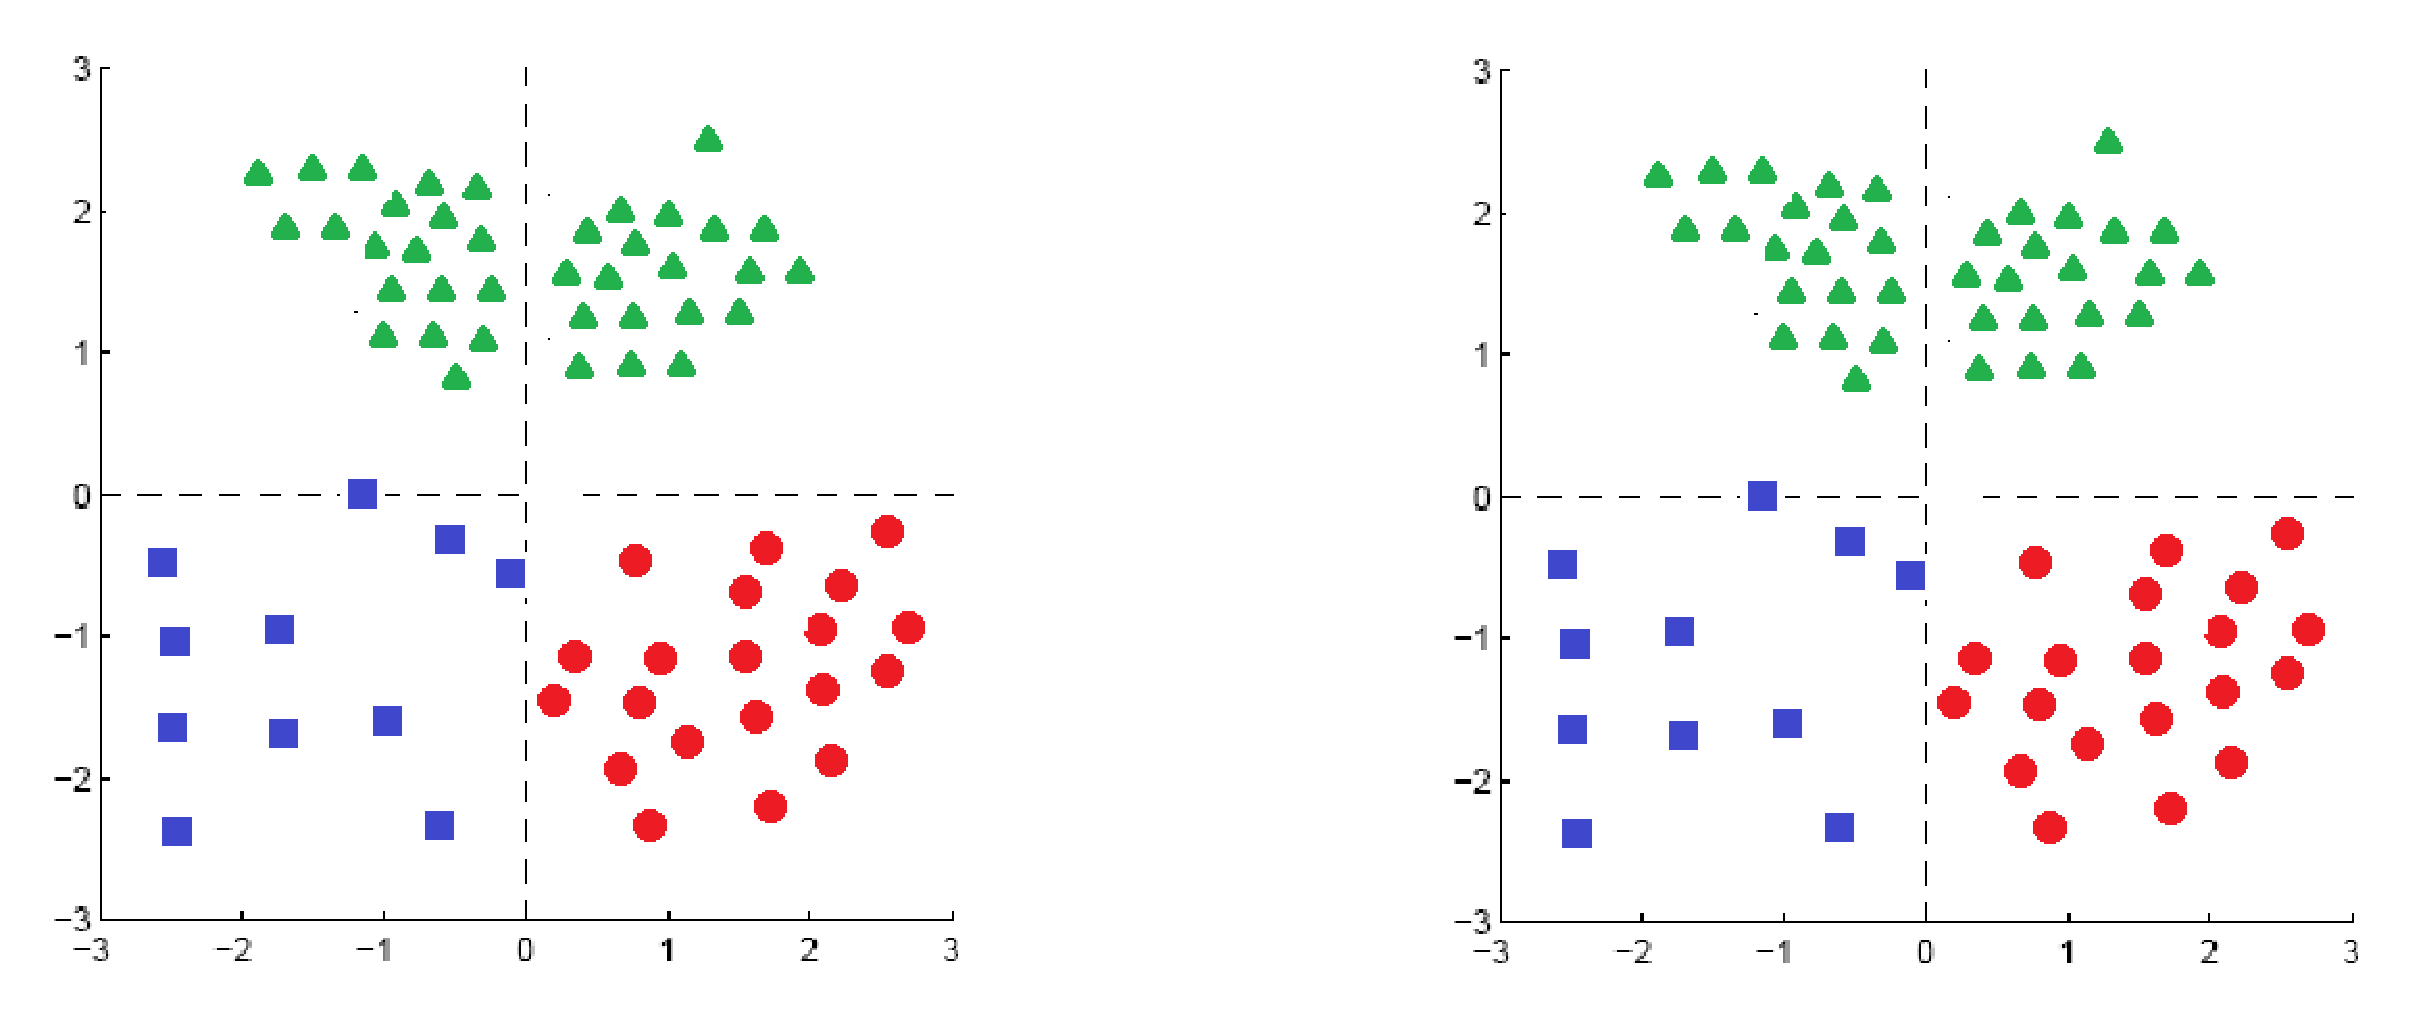
\includegraphics[scale=0.40]{imagens/npc.eps}
\caption{Exemplo do NPC}
\end{figure}

Al�m de possuir vantagens gerais como a diminui��o do espa�o de armazenamento e redu��o de esfor�o computacional para classifica��o, a sele��o de prot�tipos pode ainda aumentar o desempenho do classificador. Esta melhora acontece com a elimina��o de ru�dos e outliers, pois os prot�tipos aumentam a capacidade de generaliza��o do classificador, levando a maiores taxas de acerto.

Algumas t�cnicas de sele��o de prot�tipos selecionam inst�ncias que pertecem ao conjunto de treinamento, ou seja, elas escolhem, dentre as inst�ncias utilizadas, aquelas que julgam ser mais apropriadas para serem prot�tipos. T�cnicas que utilizam esta abordagem s�o chamadas de puramente seletivas. Exemplos de t�cnicas seletivas s�o \textit{Edited Nearest Neighbor} \cite{enn:2011}, \textit{Condensed Nearest Neighbor} \cite{cnn:1968}, \textit{Tomek Links} e \textit{One-Sided Selection} \cite{conf/icml/KubatM97}.

Outras t�cnicas criam novos elementos durante o processo de redu��o, os prot�tipos s�o criados atrav�s de combina��o entre as inst�ncias do conjunto de original e ajustes relizados por meio de treinamento supervisionado. Estas t�cnicas s�o chamadas de criativas, entre elas est�o \textit{Learning Vector Quantization 1, 2.1 e 3} \cite{kohonen:lvq} e \textit{Self-Generating Prototypes}\cite{fayed:sgp}.

T�cnicas de sele��o de prot�tipos tamb�m podem ser classificadas como determin�sticas ou n�o deterministicas. T�cnicas determin�sticas s�o aquelas que, dada uma base de dados, sempre ser� gera o mesmo conjunto de prot�tipos, independente da ordem em que as inst�ncias de treinamento s�o apresentadas. T�cnicas n�o determin�sticas s�o aquelas que dependem da ordem das inst�ncias de treinamento, ou dependem de inst�ncias pr�-selecionadas para ajuste posterior.

Cada uma das t�cnicas de sele��o de prot�tipos aprensentam caracter�sticas pr�prias, sendo necess�rio uma an�lise do quanto cada uma destas t�cnicas � apropriada para um dado tipo de base de dados. Algumas t�cnicas removem inst�ncias redundantes, outras, removem inst�ncias que est�o na fronteira de classifica��o, e outras fazem uma combina��o das duas abordagens. Detalhes de algumas destas t�cnicas ser�o mostrados no pr�ximo cap�tulo.

\subsection{Bases Desbalanceadas}

Em v�rias situa��es do mundo real, os classificadores precisam ser treinados com bases de dados que possue muito mais inst�ncias de uma de uma classe do que das outras classes, tais bases de dados s�o chamadas de bases desbalanceadas. Quanto maior a diferen�a entre a quantidade de inst�ncias de cada classe, maior o n�vel de desbalanceamento da base.

Quando treinados com bases de dados desbalanceadas, classificadores sofrem uma redu��o da performace, e normalmente tendem a classificar mais padr�es com as classes marjorit�rias. Este � um problema grave, visto que, normalmente, a classifica��o de inst�ncias da classe minorit�ria � que s�o mais importantes (como exemplo, informa��es sobre doen�as) \cite{conf/icml/HulseKN07}.

Da mesma forma que classificadores podem ser prejudicados por um desbalanceamento, t�cnicas de sele��o de prot�tipos podem sofrer da mesma forma, selecionando muitas inst�ncias da classe marjorit�ria e poucas, ou nenhuma, da classe minorit�ria.

\section{Objetivo}

O objetivo deste trabalho � expor algumas t�cnicas de sele��o de prot�tipos e avaliar seu desempenho em bases desbalanceadas. A avalia��o de desempenho se refere a taxa de acerto utilizando bases de dados reais, e a disposi��o dos prot�tipos por meio de bases artificiais de diferentes n�veis de desbalanceamento e sobreposi��o de classes.

Para que o trabalho seja mais objetivo, apenas os exemplos mais interessante de cada t�cnica de sele��o de prot�tipos ser�o enfatizados, citando as maiores vantagens e desvantagens de cada uma delas.

No final do trabalho, ser� poss�vel identificar quais t�cnicas s�o mais apropriadas para bases de dados desbalanceadas, e possivelmente propor adapta��es para otimizar algumas delas.

\section{Estrutura do Trabalho}

O restante deste trabalho possui um cap�tulo com detalhes sobre diferentes t�cnicas de sele��o de prot�tipos. Durante o cap�tulo, ser�o citadas as caracter�sticas e adapta��es j� conhecidas para tratar de bases desbalanceadas, assim como ilustra��es e algoritmos.

Logo ap�s, segue um cap�tulo mostrando casos de sucesso e falha de cada t�cnica em bases de dados artificiais, e por fim, um cap�tulo mostrado os resultados em bases de dados reais com conclus�es.

As an�lises levar�o em conta a disposi��o e a quantidade dos prot�tipos resultantes de cada t�cnica. Al�m disso, ser� calculada a taxa de acerto dos prot�tipos em rela��o ao pr�prio conjunto de treinamento para analisar a representatividade. Por fim, cada t�cnica ser� executada em bases de dados reais, onde ser� utilizada \textit{K-Fold Cross-Validation} para calcular a taxa de acerto m�dia de cada t�cnica.

% !TEX encoding = ISO-8859-1
\chapter{Web Ontology Language: OWL}
\label{ch:webontologylanguageowl}

In order to describe the connection method as a formal inference system (in section 4), and the positive matricial normal form used in it, we will briefly describe the notation we use for first order logic, before examining the method. We are presuming readers to be acquainted to first order logic.

\section{Definition 1 (First-order logic syntax).}
The alphabets given by table 1 compose the FOL syntax notation.	? Table 1. First order logic syntax notation.
% !TEX encoding = ISO-8859-1
\chapter{T�cnicas de Sele��o de Prot�tipos}
% \label{ch:tecnicasdeselecaodeprototipos}

Neste cap�tulo, ser�o mostradas as t�cnicas de sele��o de prot�tipos abordadas neste trabalho. Cada uma das sess�es abaixo abordar� uma t�cnica, ser� mostrado o conceito da t�cnica, assim como o pseudo-c�digo e as caracter�sicas de cada uma destas t�cnicas.

\section{ENN}

Edited Nearest Neighbor Rule\cite{enn:2011} � uma t�cnica de sele��o de prot�tipos puramente seletiva proposta por Wilson em 1976. De uma forma geral, esta t�cnica foi projetada para funcionar como um filtro de ru�dos, ela elimina pontos na regi�o de fronteira, regi�o de alta susceptibilidade a erros, e com isso elimina ru�dos.\

Por atuar apenas na regi�o de fronteira, esta t�cnica possui uma baixa capacidade de redu��o, deixando as inst�ncias que n�o se encontram na regi�o de fronteira intactas, exceto pelos ru�dos extremos.\

Uma desvantagem desta t�cnica � que ela possui uma baixa capacidade de redu��o de elementos, visto que ela n�o elimina redund�ncia.

Segue abaixo o algoritmo da execu��o do ENN e, logo ap�s, alguns coment�rios sobre este algoritmo.

\begin{algorithm}
\caption{ENN}
\label{pseudocode_enn}
\begin{algorithmic}[1]
\REQUIRE {$list$: uma lista}
\FORALL {inst�ncia $e_i$ da base de dados original}
\STATE Aplique o KNN sobre $e_i$
\IF {$e_i$ foi classificado erroneamente}
\STATE salve $e_i$ em $list$
\ENDIF
\ENDFOR
\STATE Remova da base de dados todos os elementos que est�o em $list$
\end{algorithmic}
\end{algorithm}

O valor de K pode variar de acordo com o tamanho da base de dados, por�m, tipicamente, utiliza-se o valor de K=3. Tipicamente, O valor de K � inversamente proporcional a quantidade de inst�ncias que ser�o eliminadas, ou seja, para que o filtro elimine todos os poss�veis ru�dos, deve-se utilizar K=1.

%% TODO COLOCAR ALGUMA FIGURA PARA EXEMPLIFICAR
%% TODO EXPLICAR A FIGURA

Uma vantagem do ENN � que ele independe da ordem que a base de dados foi apresentada, ou seja, o ENN aplicado a uma base de dados, com o mesmo valor de K, sempre ter� o mesmo resultado.

%% TODO CITAR DESVANTAGENS DO ENN 

\section{CNN}

Condensed Nearest Neighbor \cite{cnn:1968} � uma t�cnica de sele��o de prot�tipos puramente seletiva que tem como objetivo eliminar informa��o redundante. Diferentemente do ENN \cite{enn:2011}, o CNN n�o elimina inst�ncias nas regi�es de fronteira, a t�cnica mant�m estes elementos pois estes que "s�o importantes" para distinguir entre duas classes.

A ideia geral do CNN � encontrar o menor subconjunto da base de dados original que, utilizando o 1-NN, classifica todos os padr�es da base de dados original corretamente. Fazendo isso, o algoritmo elimina os elementos mais afastados da regi�o de indecis�o, da fronteira de classifica��o.

O algoritmo do CNN ser� mostrado abaixo, e logo ap�s, coment�rios a respeito do mesmo.

\begin{algorithm}
\caption{CNN}
\label{pseudocode_cnn}
\begin{algorithmic}[1]
\REQUIRE {$list$: uma lista}
\STATE Escolha um elemento de cada classe $aleatoreamente$ e coloque-os em $list$
\FORALL {inst�ncia $e_i$ da base de dados original}
\STATE Aplique o KNN sobre $e_i$ utilizando os elementos em $list$ para treinamento
\IF {$e_i$ foi classificado erroneamente}
\STATE salve $e_i$ em $list$
\ENDIF
\ENDFOR
\STATE Remova da base original todos os elementos que n�o est�o em $list$
\end{algorithmic}
\end{algorithm}

Podemos observar que este algoritmo possui uma abordagem diferente do ENN, por exemplo, pois ele come�a com um conjunto m�nimo de inst�ncias (uma de cada classe) e depois adiciona inst�ncias conforme a necessidade de mant�-las para que todos os elementos da base de dados original sejam classificados corretamente.

Uma coisa que pode-se observar no algoritmo, � a palavra $aleatoriamente$, o que significa que o CNN aplicado numa mesma base de dados com um mesmo valor de K para o KNN, nem sempre resulta nos mesmos prot�tipos. O primeiro fato para que isso ocorra � a sele��o aleat�ria dos prot�tipos iniciais. Existem algumas adapta��es para o CNN, onde os prot�tipos iniciais s�o escolhidos utilizando t�cnicas como o SGP\cite{fayed:sgp} para obter as inst�ncias mais centrais. Modifica��es no CNN s�o muito comuns \cite{cnn:1976}, por�m, mesmo com estas modifica��es, o CNN ainda n�o � determin�stico, pois a ordem em que as inst�ncias s�o classificadas afeta o resultado final.

%% TODO COLOCAR ALGUMA FIGURA PARA EXEMPLIFICAR
%% TODO EXPLICAR A FIGURA

Para o caso de estudo abordado neste trabalho, o CNN pode ser utilizado de forma adaptada. A adapta��o consiste em manter todos os elementos da classe minorit�ria e o m�nimo poss�vel da classe marjorit�ria. O pr�prio CNN se encarrega de remover os elementos redundantes da classe marjorit�ria, assim, basta apenas selecionar todos os elementos da classe minorit�ria aos prot�tipos iniciais.
Segue abaixo o algoritmo desta adapta��o:

\begin{algorithm}
\caption{CNN para bases desbalanceadas}
\label{pseudocode_cnn}
\begin{algorithmic}[1]
\REQUIRE {$list$: uma lista}
\STATE Coloque todos os elementos da classe minorit�ria em $list$
\FORALL {inst�ncia $e_i$ da base de dados original}
\STATE Aplique o KNN sobre $e_i$ utilizando os elementos em $list$ para treinamento
\IF {$e_i$ foi classificado erroneamente}
\STATE salve $e_i$ em $list$
\ENDIF
\ENDFOR
\STATE Remova da base original todos os elementos que n�o est�o em $list$
\end{algorithmic}
\end{algorithm}

Com o algoritmo CNN adaptado para bases desbalanceadas, os elementos redundantes da classe marjorit�ria s�o removidos, e todos os elementos da classe minorit�ria s�o mantidos. Esta adapta��o do CNN ir� reduzir a base de dados, ocasionando as vantagens de redu��o, e ainda reduzir� o desbalenceamento da base.


\section{Tomek Links}

Mantendo a mesma linha do ENN, Tomek Links � uma t�cnica de sele��o de prot�tipos puramente seletiva que elimina os elementos das regi�es de fronteiras e inst�ncias com probabilidade de ser ru�do. Tomek Links podem ser definidos da seguinte forma: Dadas duas inst�ncias $e_i$ e $e_j$, o par \textit{($e_i$, $e_j$)} � chamado de Tomek Link se n�o existe nenhuma inst�ncia $e_k$, tal que, para todo $e_k$ \textit{dist($e_i$,$e_j$) < dist($e_i$,$e_k$)} e \textit{dist($e_i$,$e_j$) < dist($e_j$,$e_k$)}. Segue abaixo o algor�tmo detalhado:

\begin{algorithm}
\caption{Seleciona Tomek Links}
\label{pseudocode_cnn}
\begin{algorithmic}[1]
\REQUIRE {$list$: uma lista}
	\FORALL {inst�ncia $e_i$ da base de dados original}
		\STATE $e_j$ = inst�ncia mais pr�xima de $e_i$
		\IF {inst�ncia mais p�oxima de $e_j$ for $e_i$}
			\IF {classe de $e_i$ for diferente da classe de $e_j$}
				\STATE salve o par \textit{($e_i$, $e_j$)} em $list$
			\ENDIF
		\ENDIF
	\ENDFOR
	\STATE Retorne os pares em $list$, os Tomek Links
\end{algorithmic}
\end{algorithm}



Os Tomek Links representam elementos da regi�o de fronteira e prov�veis ru�dos, e a t�cnica de sele��o de prot�tipos consiste em remover os Tomek Links da base de dados original. Segue abaixo o algoritmo da sele��o de prot�tipos:



\begin{algorithm}
\caption{Tomek Links}
\label{pseudocode_cnn}
\begin{algorithmic}[1]
\REQUIRE {$list$: uma lista}
\STATE $list$ = $Seleciona Tomek Links$ da base original
	\FORALL {\textit{($e_i$, $e_j$)} em $list$}
		\STATE remova $e_i$ da base original
		\STATE remova $e_j$ da base original
	\ENDFOR
	\STATE Retorne a base original filtrada
\end{algorithmic}
\end{algorithm}



Enquanto o CNN remove os elementos que est�o longe da regi�o de indecis�o, o Tomek Links remove os elementos que est�o pr�ximos desta regi�o, o que causa uma maior separa��o entre as classes.



%% TODO FIGURA PARA TOMEK LINKS
%% EXPLICAR FIGURA



Observa-se facilmente que os Tomek Links pode remove todas as inst�ncias da fronteira, inclusive as inst�ncias da classe minorit�ria, assim sendo, uma poss�vel adapta��o dos Tomek Links � eliminar apenas os elementos das classes marjorit�rias. Nesse caso, ainda ocorreria uma separa��o entre as classes, mas apenas as inst�ncias da classe marjorit�ria seriam removidos, dimunuindo assim o n�vel de desbalanceamento. Segue abaixo o algoritmo desta adapta��o:



\begin{algorithm}
\caption{Tomek Links}
\label{pseudocode_cnn}
\begin{algorithmic}[1]
\REQUIRE {$list$: uma lista}
	\STATE $list$ = $Seleciona Tomek Links$ da base original
	\FORALL {\textit{($e_i$, $e_j$)} em $list$}
		\IF {$e_i$ for da classe marjorit�ria}
			\STATE remova $e_i$ da base original
		\ENDIF
		\IF {$e_j$ for da classe marjorit�ria}
			\STATE remova $e_j$ da base original
		\ENDIF
	\ENDFOR
	\STATE Retorne a base original filtrada
\end{algorithmic}
\end{algorithm}



Com esta adapta��o, a classe minorit�ria � mantida, evitando o aumento do desbalanceamento ou a remo��o por alta probabilidade de ru�do.



\section{LVQ}
\subsection{LVQ 1}
\subsection{LVQ 2.1}
\subsection{LVQ 3}
\section{SGP}
\section{SGP 2}
\section{CCNN}



% !TEX encoding = ISO-8859-1
\chapter{Conclus�o}
% \label{ch:introducao}

\section{Considera��es Finais}

	Com os experimentos realizados conclui-se que t�cnicas como o \textit{Edited Nearest Neighbor} e \textit{Tomek Links} em suas vers�es originais s�o eficientes para remo��o de ru�dos, por�m, para bases desbalanceadas ela pode remover todas as inst�ncias da classe minorit�ria, tornando a base invi�vel para qualquer classificador. Para uso destas t�cnicas, recomenda-se uma adapta��o para n�o remover inst�ncias da classe minorit�ria.

	O \textit{Condensed-Nearest Neighbor} pode ser eficiente, dependendo da sobreposi��o de classes. Em casos onde as classes est�o bem separadas, o uso do CNN s� deve ser feito caso o classificador considere apenas a inst�ncia mais pr�xima. Caso o classificador seja um 3-NN, esta t�cnica pode deixar apenas um prot�tipo da classe minorit�ria, tornando-a invi�vel, mesmo para pr�-processamento. Para o CNN uma boa op��o � utilizar sua vers�o adaptada.

	A t�cnica que se mostrou muito eficiente foi o \textit{One-Sided Selection}. Esta t�cnica foi eficiente em identificar a classe minorit�ria em todos os experimentos, independente do n�vel de sobreposi��o e desbalanceamento. Por�m, esta t�cnica possui um baixo poder de redu��o de inst�ncias, sendo recomendado utilizar o OSS como t�cnica de pr�-sele��o de prot�tipos.

	Assim como o OSS, as vers�es do \textit{Learning Vector Quantization}, ao reduzir o n�vel de desbalanceamento favorece a classe minorit�ria. Independente do n�vel de sobreposi��o, esta t�cnica se mostrou eficiente. Um defeito desta t�cnica � que ela possui muitos par�metros, ent�o, a escolha dos valores adequados pode tornar o processo de treinamento lento.

	As duas vers�es do \textit{Self-Generating Prototypes} s�o muito eficientes para bases com baixo n�vel de desbalanceamento e sobreposi��o. Mas ambas as vers�es possuem um p�ssimo desempenho em classificar inst�ncias da classe minorit�ria quando existe um alto desbalanceamento e sobreposi��o de classes. Recomenda-se n�o utilizar esta t�cnicas com fator de generaliza��o para evitar a elimina��o da classe minorit�ria em bases desbalanceadas.

	Ap�s analisar todas as t�cnicas, percebe-se que aquelas que tratam a classe minorit�ria de forma especial possuem um melhor desempenho em identificar esta classe do que t�cnicas que tratam todas as classes igualmente. Ent�o, recomenda-se o uso de t�cnicas que diminuam o desbalanceamento antes de aplicar t�cnicas tradicionais de sele��o de prot�tipos, para que haja efici�ncia em identificar a classe minorit�ria.

\section{Trabalhos Futuros}

	Percebendo que t�cnicas adaptadas para classes desbalanceadas com o \textit{One-Sided Selection} possuem um bom desempenho, � de se esperar que o \textit{Self-Generating Prototypes} que trate as classes marjorit�ria e minirit�ria de formas distintas seja tamb�m eficiente.

	O SGP 1 e 2 possuem um alto poder de redu��o de inst�ncias e se mostraram muito eficiente em bases com baixo n�vel de desbalanceamento. Para trabalhos futuros, uma adapta��o no SGP pode gerar uma t�cnica que mantenha as caracter�sticas de representa��o de classes, mas que promova uma redu��o no desbalanceamento, pode ser muito eficiente.

	Uma adapta��o percept�vel atrav�s dos experimentos deste trabalho � utilizar fatores de generaliza��o diferentes para a classe marjorit�ria e para minorit�ria. Isso pode ser feito utilizando o maior grupo de uma classe $C$ para eliminar um grupo da classe $C$, e n�o o maior grupo da base. Para o SGP 2, as fases de $Merge$ e $Pruning$ podem ser feitas apenas com grupos da classe marjorit�ria.

	Com estas adapta��es sugeridas, o SGP ter� as mesmas caracter�sticas de redu��o de inst�ncias e representatividade das classes, mas favorecer� a identifica��o da classe minorit�ria, assim como o OSS.








%% Parte p�s-textual
\backmatter

\appendix
% \include{apendice1}

% Bibliografia
\nocite{*}
\bibliographystyle{alpha}
\bibliography{bibliografia/bibliografia}

% \colophon % UFPEThesis reference

\end{document}
